\chapter{Week 1 - Lecture 2: Innovation and production }
\textit{7-09-2017 \\
Carolina Castaldi \\} 
\\
This lecture introduces some basic economic ideas related to the introduction of innovation in production, in particular process innovation. Different forms of innovating in production will be related to different groups of sectors in the economy (the so-called Pavitt taxonomy).
\\
\section{How do firms profit from innovation?}
\begin{enumerate}
\item Product innovation: increasing quality of products to be able to charge higher prices;
\item Process innovation: improve production to be able to lower costs.
\end{enumerate}

\section{What sort of production costs are there?}
\begin{itemize}
\item \textsc{Total cost} (TC): the total economic cost of production, consisting of fixed and variable costs;
\item \textsc{Fixed cost} (FC): cost that does not vary with the level of output and that can be eliminated only by shutting down;
\item \textsc{Variable cost} (VC): cost that varies as output varies;
\item \textsc{Sunk cost} (SC): cost have been incurred and cannot be recovered.
\end{itemize}

\section{What does economies of scale mean?}
Economies of scale is the cost advantage that arises with increased output of a product. Economies of scale arise because of the inverse relationship between the quantity produced and per-unit fixed costs; i.e. the greater the quantity of a good produced, the lower the per-unit fixed cost because these costs are spread out over a larger number of goods.
\subsection{Sources of economies of scale}
\begin{itemize}
\item Indivisibilies and spreading of fixed / sunked costs in production: in capital-intensive production, in sectors with large overhead/inventories, in R\&D intensive sectors.
\item Purchasing economies
\item Advertising economies
\item The square-cube rule: mathematical principle, applied in a variety of scientific fields, which describes the relationship between the volume and the area as a shape's size increases or decreases. A shape grows in size, its volume grows faster than its surface area. 
\end{itemize}

\section{Which type of costs are most prominent in computer -, pharmaceutical and airline industry?}
\begin{itemize}
\item \textsc{Computer industry}: Variable costs / Sunk costs with economies of scale in production;
\item \textsc{Pharmaceutical industry}: Sunk costs with economies of scale in R\&D and in marketing; 
\item \textsc{Airline industry}: Fixed costs with economies of scale in production. 
\end{itemize}

\section{What is diseconomies of scale?}
In microeconomics, diseconomies of scale are the cost disadvantages that firms and governments accrue due to increase in firm size or output, resulting in production of goods and services at increased per-unit costs. This typically follows the law of diminishing returns, where further increase in size of output will result in even greater increase in average cost. This concept is the opposite of economies of scale

\begin{figure}[h]
\begin{center}

\includegraphics{DES}
\end{center}
\end{figure}

\section{Process innovation and costs}
\begin{enumerate}
\item A reduction in fixed costs with no change in marginal costs;
\item A reduction in marginal costs, with no change in fixed costs;
\item A reduction in marginal costs accompanied by an increase in fixed costs
\end{enumerate}

\section{What is the Learning Curve?}
A concept developed by the Boston Consulting Group in the 1960's. It is representative of a consistent relationship between the cost of production and the cumulative production quantity (total quantity produced from the first unit to the last). The experience curve implies that the more experience a firm has in producing a particular product, the lower are its costs.

\begin{itemize}
\item 
\end{itemize}

\begin{figure}[h]
\begin{center}
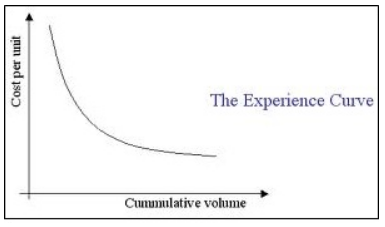
\includegraphics{LearningCurve}
\end{center}
\end{figure}

\section{What is Moore's law?}
Moore's law is the observation that the number of transistors in a dense integrated circuit doubles approximately every two years. The observation is named after Gordon Moore, the co-founder of Fairchild Semiconductor and Intel, whose 1965 paper described a doubling every year in the number of components per integrated circuit, and projected this rate of growth would continue for at least another decade.

\section{Test}
Dit is een test. Hoe werkt dit? Werkt het goed?





